\clearpage
%//==============================--@--==============================//%
\subsection[4.2 Problema de decisão]{$\rightarrow$ Problema de decisão}
\label{subsec:optimum-receiver-coherent-detection}

Nesta secção é analisado o problema de reconhecer um sinal escolhido aleatoriamente (com probabilidades conhecidas) de um conjunto finito conhecido $\{s_i(t)\}_{i=1}^{M}$ após ser perturbado por um processo de ruído $n(t)$ independente do sinal e adicionado a este. 

Refinadamente, o problema é decidir, qual dos sinais, $s_1(t)$, $s_2(t)$, $\dots$, $s_M(t)$, levou à obtenção do sinal $r(t)$, quando se sabe que $r(t)$ tem a forma
$$
    r(t) = s_i(t) + n(t)
$$
para algum $i$, $1 \leq i \leq M$. Será assumido que $n(t)$ é um processo gaussiano, com densidade espectral de potência $N_0/2$. Os sinais têm energia finita e duração finita. Assume-se que $s_i(t)$, $1 \leq i \leq M$, são definidos num intervalo $0 \leq t \leq T$ e que $r(t)$ é observado no mesmo intervalo. Definimos então o \underline{problema de decisão}.

%//==============================--@--==============================//%
\subsubsection[4.2.1 Caracterização estatística da saída do correlador]{$\rightarrow$ Caracterização estatística da saída do correlador}

Seja $r_j$ definido como
\begin{align*}
    r_j &\delequal \int_{0}^{T} r(t) \phi_j(t)\, dt,\qquad j=1,2,\dots,N \\
    &= s_{ij} + n_{j}
\end{align*}
em que 
$$
    n_j \delequal \int_{0}^{T} n(t) \phi_j(t)\, dt,\qquad j=1,2,\dots,N
$$

\noindent O valor médio do valor observado do processo estocástico é dado por
\begin{align*}
    \mu_{r_j} &= \mathbb{E}[r_j] \\
    &= \mathbb{E}[s_{ij} + n_j] \\
    &= s_{ij} + \mathbb{E}[n_j] = s_{ij}
\end{align*}

\noindent A variância pode ser calculada através da definição
\begin{align*}
    \sigma_{r_j}^2 &= \text{Var}[r_j] \\
    &= \mathbb{E}[(r_j - s_{ij})^2] \\
    &= \mathbb{E}[n_j^2] 
\end{align*}
Desta forma, de acordo com o supramencionado, é possível expandir a expressão como:
\begin{align*}
    \sigma_{r_j}^2 &= \mathbb{E}\left[ \int_{0}^{T} n(t) \phi_j(t)\, dt\, \int_{0}^{T} n(u) \phi_j(u)\, du \right] \\
    &= \int_{0}^{T} \int_{0}^{T} \phi_j(t) \phi_j(u) \mathbb{E}[n(t)n(u)] \, dt\,du
\end{align*}
Dado que 
$$
    \mathbb{E}[n(t)n(u)] = R_{n}(t,u) = \frac{N_0}{2}\, \delta(t-u)
$$
$$
    \therefore \sigma_{r_j}^2 = \frac{N_0}{2} \int_{0}^{T} \phi_j^2(t)\, dt
$$
\begin{theo}[\underline{Teorema da Irrelevância}]{def:irrelevance-theorem}\label{def:irrelevance-theorem}
    Apenas a projeção do ruído nas funções base do conjunto de sinais $\{s_i(t)\}_{i=1}^{M}$ afeta as \textit{estatísticas suficientes} do \underline{problema de decisão}; o restante ruído é irrelevante.
\end{theo}

%//==============================--@--==============================//%
\clearpage
\subsubsection[4.2.2 \textit{Optimum detector}: \textit{M} sinais reais]{$\rightarrow$ \textit{Optimum detector}: $\pmb{M}$ sinais reais no seio do ruído}
Focamo-nos então no problema enunciado no início desta secção, i.e., decidir entre as seguintes $M$ hipóteses
$$
    H_i:\quad y(t) = s_i(t) + n(t),\quad i = 1,2,\dots,M 
$$
após uma observação de $y(t)$ no intervalo de tempo $[0, T]$. Os M sinais $s_i(t)$ são conhecidos e têm energia finita, bem como duração. Através do \hyperref[def:gram-schmidt]{procedimento de Gram-Schmidt}, é possível determinar um conjunto de sinais ortonormais $(\phi_j(t))_{j=1}^{N}$, $N \leq M$, tal que cada $s_i(t)$, $i=1,2,\dots,M$, possa ser representado como uma combinação linear destas bases. Consideremos também uma sequência completa de sinais ortonormais cujos primeiros $N$ elementos são $\phi_1(t)$, $\dots$, $\phi_N(t)$. Denotemos esta sequência por $(\phi_j(t))_{j=1}^{+\infty}$, e definimos
$$
    s_{ij} \delequal \int_{0}^{T} s_i(t)\phi_j(t)\, dt,\quad i=1,2,\dots,M,\quad j=1,2,\dots 
$$
e $n_j$, $Y_j$ do mesmo modo. O \underline{problema de decisão} pode ser formulado da seguinte forma discreta. Escolher entre as $M$ hipóteses
$$
    H_i:\quad (Y_j)_{i=1}^{+\infty} = (s_{i1}+n_1, s_{i2}+n_2, \dots, s_{iN}+n_N, n_{N+1}, n_{N+2},\dots)
$$
$i=1,2,\dots,M$, com base nas observações das VA's $Y_1$, $Y_2$, $\dots$. Dado que as componentes de ruído $n_{N+1}$, $n_{N_2}$,$\dots$, são independentes de $v_1$, $\dots$, $v_N$, e das hipóteses, as observações $Y_{N+1}$, $Y_{N+2}$,$\dots$, não acrescentam informação nenhuma ao processo de decisão. Portanto podemos basear-nos somente na observação de $Y_1$, $Y_2$,$\dots$, $Y_N$. Definindo os vetores linha $[N \times 1]$ $\pmb{Y} \delequal [Y_1,Y_2,\dots,Y_N]$, $\pmb{n} \delequal [n_1,n_2,\dots,n_N]$, e $\pmb{s}_i \delequal [s_{i1},s_{i2},\dots,s_{iN}]$, $i=1,2,\dots,M$, é possível reduzir a decisão para a forma vetorial 
$$
    H_i:\quad \pmb{Y} = \pmb{s}_i + \pmb{n},\quad i=1,2,\dots,M
$$
Desta forma, o \textit{optimum detector} procura funcionar de tal forma que
$$
    \texttt{escolher } H_i \texttt{ se } \pmb{y} \in S_i
$$
onde $\pmb{y}$ denota o valor observado do vetor aleatório $\pmb{Y}$, e $S_1$, $S_2$,$\dots$, $S_M$ são as partições do espaço $N$-dimensional, tal que esta regra dê azo à menor probabilidade de erro média
$$
    P(e) = 1 - \sum_{i=1}^{M} p_i\, \int_{S_i} f_{\pmb{Y}|H_i}\left( \pmb{z} | H_i \right)\, d\pmb{z}
$$
em que $p_i \delequal P\{H_i\}$, $i=1,2,\dots,M$. É verificado que $P(e)$ é minimizado se cada $S_i$ for escolhido de forma a que
$$
    \pmb{z} \in S_i \texttt{ se, e somente se, } p_i\, f_{\pmb{Y} | H_i}(\pmb{z}|H_i) = \max_{j} p_j\, f_{\pmb{Y} | H_j}(\pmb{z}|H_j)
$$
Obtemos então o critério de decisão de \underline{\textit{maximum a posteriori}} (MAP). Neste caso, as $M$ regiões $S_i$ são denominadas por \textit{regiões de decisão} MAP. No caso especial em que as hipóteses $H_i$ são equiprováveis, i.e., $p_i = 1/M$, obtém-se
$$
    \pmb{z} \in S_i \texttt{ se, e somente se, } f_{\pmb{Y} | H_i}(\pmb{z}|H_i) = \max_{j} f_{\pmb{Y} | H_j}(\pmb{z}|H_j)
$$
que corresponde à regra de decisão de \underline{\textit{máxima verosimilhança}} (ML). Apesar de apenas minimizar $P(e)$ para hipóteses $H_i$ equiprováveis, é o método de deteção mais utilizado, e será onde confinaremos a nossa deteção.

Definindo a hipótese auxiliar
$$
    H_0:\quad \pmb{Y} = \pmb{n},
$$
a condição de ML pode ser reescrita como
$$
    \pmb{z} \in S_i \texttt{ se, e somente se, } \Lambda_i(\pmb{z}) = \max_{i} \Lambda_j(\pmb{z})
$$
onde definimos os \textit{likelihood ratios}
$$
    \Lambda_i(\pmb{z}) \delequal \frac{f_{\pmb{Y} | H_i}(\pmb{z}|H_i)}{f_{\pmb{Y} | H_0}(\pmb{z}|H_0)}
$$
Deste modo, a regra de decisão ML é
$$
    \texttt{escolher } H_i \texttt{ se } \Lambda_i(\pmb{y}) = \max_{i} \Lambda_j(\pmb{y})
$$
onde $\pmb{y}$ representa, como anteriormente, o valor observado de $\pmb{Y}$. Isto é, o detetor ML calcula os $M$ \textit{likelihood ratios} $\Lambda_1(\pmb{y})$, $\Lambda_2(\pmb{y})$,$\dots$,$\Lambda_M(\pmb{y})$, e escolhe a hipótese que corresponde ao maior de entre a seleção. Observando que $pmb{Y}$ é um vetor aleatório gaussiano com valor médio $\pmb{s}_i$ (ou zero, para $i=0$), componentes independentes, e variância $N_0/2$ para cada componente, temos, para $i=1,2,\dots,M$,
$$
    \Lambda_i(\pmb{z}) = \frac{\exp[-(1/N_0)\, |\pmb{y}-\pmb{s}_i|^2]}{\exp[-(1/N_0)\, |\pmb{y}|^2]}
$$
onde $|\pmb{x}|^2 = \pmb{x}\pmb{x}^T = \sum_{j=1}^{N} x^2_j$ (módulo ao quadrado do vetor $\pmb{x}$). Definindo os \textit{log-likelihood ratios}
$$
    \lambda_i(\pmb{y}) \delequal \ln{\Lambda_i(\pmb{y})}
$$
permite reduzir a condição para a simples forma
$$
    \texttt{escolher } H_i \texttt{ se } \pmb{y}\pmb{s}_i^T - \frac{1}{2} |\pmb{s}_i|^2 = \max_{i}\left\{ \pmb{y}\pmb{s}_j^T - \frac{1}{2} |\pmb{s}_j|^2 \right\} 
$$
Uma expressão mais familiar para o \textit{log-likelihood ratio} pode ser dada por 
\begin{mdframed}
$$
    \therefore \lambda_i(y) = \frac{2}{N_0} \int_{0}^{T} y(t) s_i(t)\, dt - \frac{1}{N_0} \int_{0}^{T} s_i^2(t)\, dt,\qquad i=1,2,\dots,M
$$
\end{mdframed}

\begin{figure}[ht] 
    \begin{subfigure}[b]{0.5\linewidth}
        \centering
        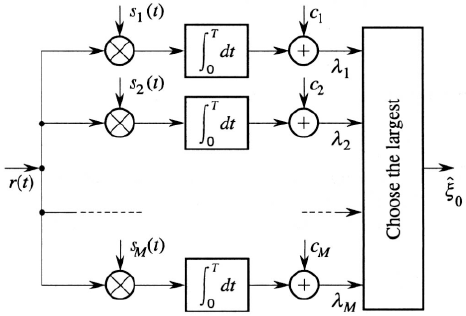
\includegraphics[width=0.9\linewidth]{img/digital/AWGN-transmission/detection-correlator.png}
        \caption{Implementação com $M$ correladores.} 
        \label{fig:detection-correlator} 
    \end{subfigure}%%
    \begin{subfigure}[b]{0.5\linewidth}%%
        \centering
        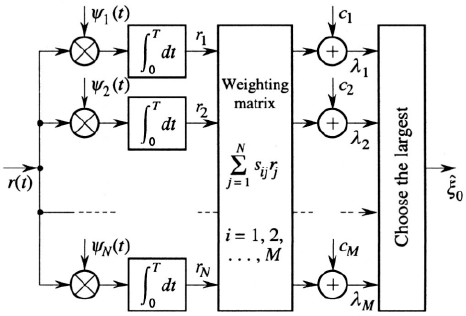
\includegraphics[width=0.9\linewidth]{img/digital/AWGN-transmission/detection-reference.png} 
        \caption{Redução de complexidade, $N \leq M$.} 
        \label{fig:detection-reference} 
    \end{subfigure}
    \caption{Implementação do recetor ótimo coerente com correladores.\cite{Benedetto1999}}
    \label{fig:} 
\end{figure}

\noindent Em que as constantes $c_i$, $i=1,2,\dots,M$, são dadas por
$$
    c_i \delequal -\frac{1}{2} \int_{0}^{T} s_i^2(t)\, dt = -\frac{1}{2} E_i
$$
onde $E_i$ denota a energia do $i$-ésimo sinal.
%Adoro-te :3
%//==============================--@--==============================//%